\section{Results}

\subsection{Evaluation of clustering methods}

The goal of this evaluation is to find an accurat clustering method for working with news articles. The most suitable algorithm will then be used for the online approach of detecting changes in a news stream based on stories.


To begin the evaluation, we first compare six different clustering methods with each other. K-means is included as a baseline, to put the scores in relation to one of the most commonly used clustering algorithms. As we can see in figure \ref{fig:different_clusterings}, HDBSCAN provides the highest accuracy, while being still being one of the fastest algorithms. Based on this data, we can assume HDBSCAN to be a good candidate to work with further. Therefore we focus on this algorithm for the rest of the evaluation to get more insight into its performance and other important properties.

\begin{figure}[h]
    \centering
    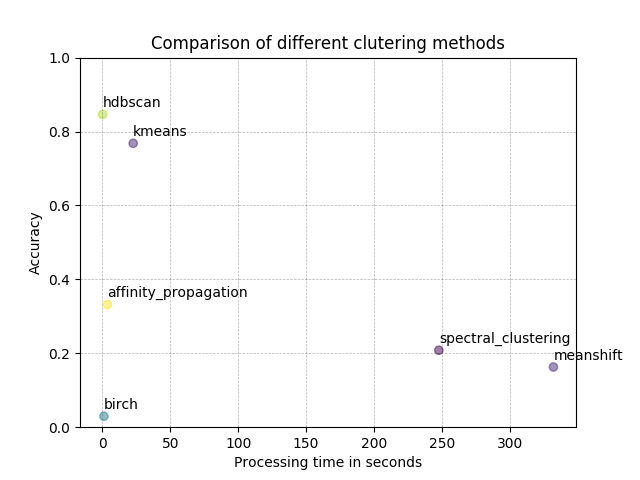
\includegraphics[width=0.5\textwidth]{different_clusterings}
    \caption{Comparison of different clustering methods with a sample size of approximately 1000 news articles}
    \label{fig:different_clusterings}
\end{figure}

% TODO Explain why HDBSCAN is better than the rest

Increasing the sample size results for both HDBSCAN and K-means in a small loss regarding the accuracy as can be seen in figure \ref{fig:accuracy_kmeans_hdbscan}. However the accuracy seems to stabilize around the 0.7 mark. The drop in the beginning is due to the fact, that for each run, we load the news articles based 

% TODO fix error in data collection

\begin{figure}[h]
    \centering
    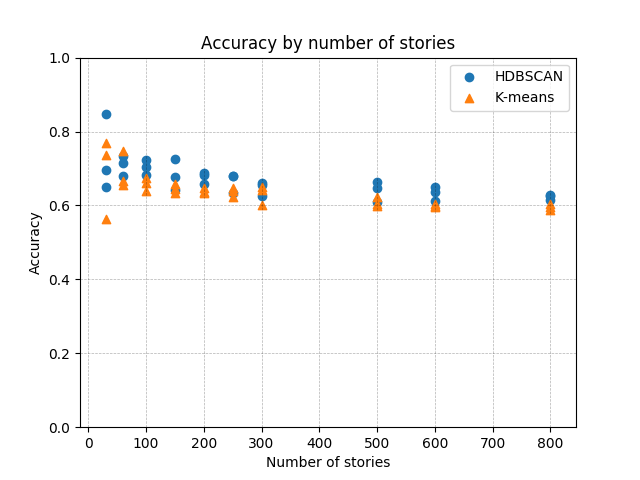
\includegraphics[width=0.5\textwidth]{accuracy_kmeans_hdbscan}
    \caption{Comparison of the average accuracy between K-means and HDBSCAN}
    \label{fig:accuracy_kmeans_hdbscan}
\end{figure}

While HDBSCAN and K-means provide a similar accuracy, the biggest difference can be noted in the processing time in relation to an increasing number of samples. K-means has a time complexity of $O(n^2)$ in contrast to HDBSCAN with a time complexity of $O(nlog(n))$, which is demonstrated by figure \ref{fig:processing_time_kmeans_hdbscan}.

\begin{figure}[h]
    \centering
    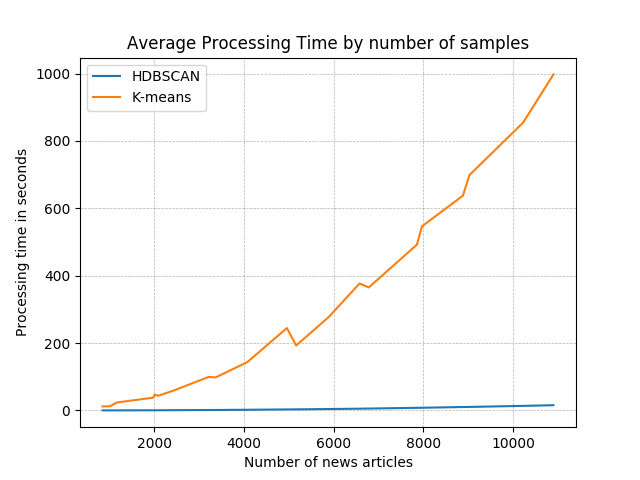
\includegraphics[width=0.5\textwidth]{processing_time_kmeans_hdbscan}
    \caption{Processing time in seconds }
    \label{fig:processing_time_kmeans_hdbscan}
\end{figure}

Figure \ref{fig:cluster_difference_samples} shows, that the difference between predicted over the true number of clusters is fairly low and appears to be roughly linear with the overall number of clusters.  

\begin{figure}[h]
    \centering
    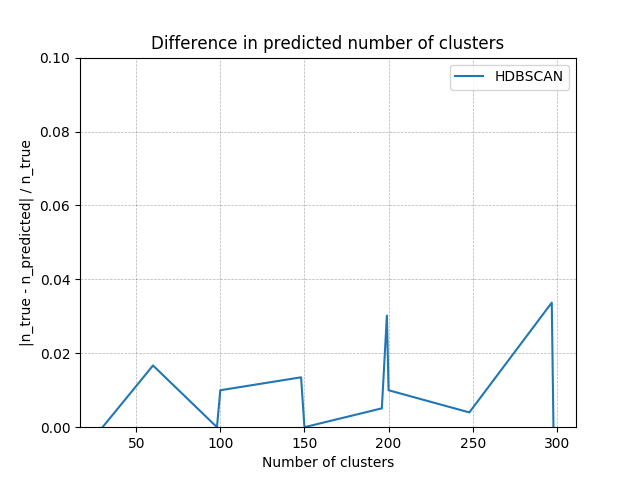
\includegraphics[width=0.5\textwidth]{cluster_difference_samples}
    \caption{Ratio of difference over predicted with true number of clusters}
    \label{fig:cluster_difference_samples}
\end{figure}

Being able to handle noise is one of the advantages of HDBSCAN has over the other previously tested clustering algorithms. It is reasonable to expect to have a lot of noise in the incoming stream of news articles, once the algorithm is applied in an online setting. However this evaluation is done with a labeled static dataset, containing a minimum amount of noise. The noise ratio shown in Figure \ref{fig:noise_ratio_samples} is much higher, than we would expect from the test data. 

\begin{figure}[h]
    \centering
    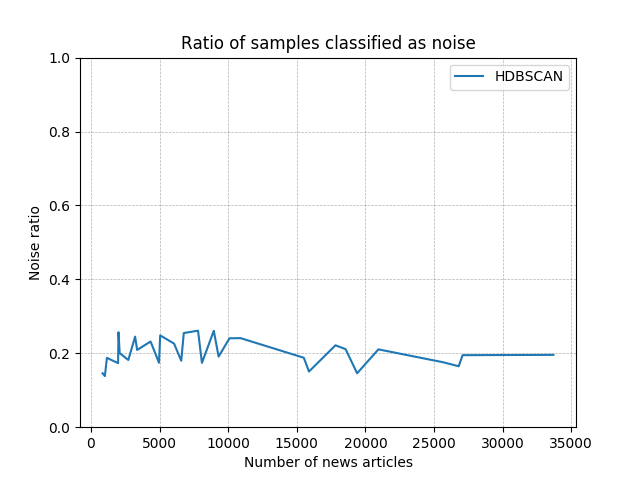
\includegraphics[width=0.5\textwidth]{noise_ratio_samples}
    \caption{Number of news articles classified as noise.}
    \label{fig:noise_ratio_samples}
\end{figure}

% Explain the high noise rate

% Show different samples

So far we have looked at data provided by the most accurate parameter combination. Figure \ref{fig:hdbscan_parameters} shows the accuracies of two essential parameters for using HDBSCAN. 

\begin{figure}[h]
    \centering
    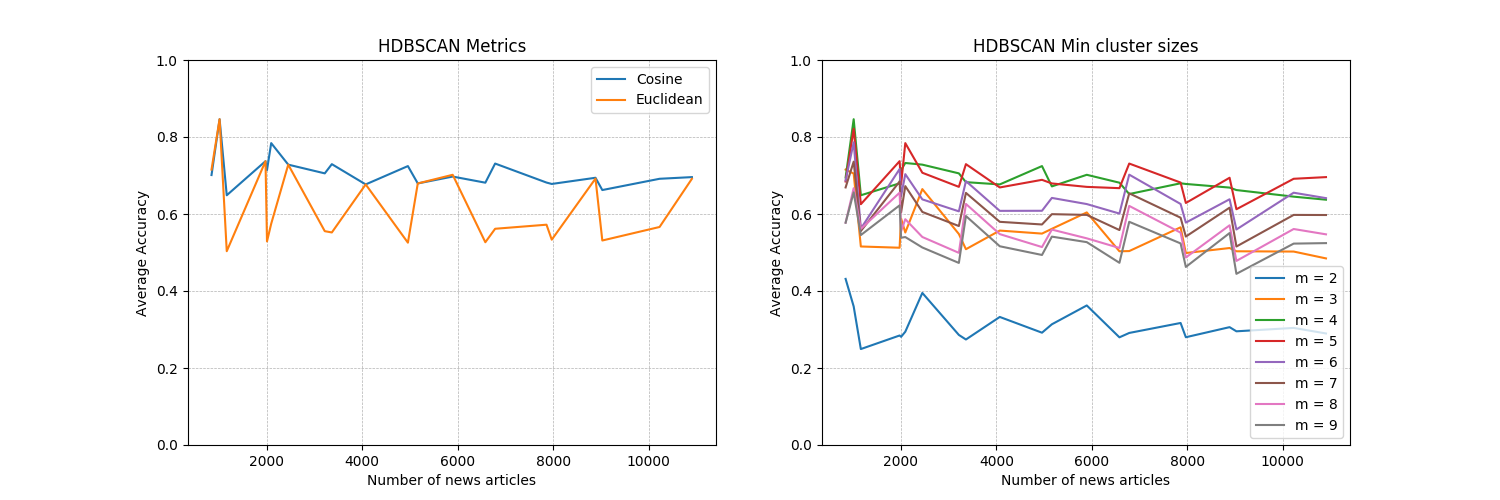
\includegraphics[width=1\textwidth]{hdbscan_parameters}
    \caption{Accuracies for different parameters}
    \label{fig:hdbscan_parameters}
\end{figure}
